\documentclass[10pt,a4paper]{article}
\usepackage{arabtex}
\usepackage[OT1,T1,LFE,LAE]{fontenc}
\usepackage[utf8]{inputenc}
\usepackage[arabic,english,farsi]{babel}
\usepackage{amsmath,amsfonts} % Math packages
\usepackage{amssymb}

\usepackage{multicol}

\usepackage{graphicx}
\usepackage{color}
\usepackage{float}
\usepackage{sidecap}
\usepackage{anysize}
\marginsize{2cm}{2cm}{2cm}{2cm}

\usepackage{listings}

\usepackage{appendix}

\usepackage[colorlinks=true,plainpages=true,citecolor=blue,linkcolor=blue,urlcolor=cyan]{hyperref}

%%% Equation and float numbering
\numberwithin{equation}{section}
\numberwithin{figure}{section}
\numberwithin{table}{section}


\newcommand{\horrule}[1]{\rule{\linewidth}{#1}} 	% Horizontal rule

\newcommand{\titleText}{STP and Switch \\ Laboratory Manual}

\title{
\normalsize In the name of Allah\\
\vspace{10pt}
\LARGE\FR{بسم \allah الرحمن الرحیم}
\vspace{10pt}
\begin{center}
	%	\newcommand{\HRule}{\rule{\linewidth}{0.5mm}}
	\begin{minipage}{0.48\textwidth} \begin{flushleft}
			
\includegraphics[height=64pt,width=64pt]{../img/logo.png}
	\end{flushleft}\end{minipage}
	\begin{minipage}{0.48\textwidth} \begin{flushright}
			
\includegraphics[height=64pt]{../img/eng-logo.png}
	\end{flushright}\end{minipage}
\end{center}
\vspace*{-64pt}
%	\horrule{0.5pt} \\[0.4cm]
	\huge \titleText\\
\vspace{40pt}
%	\horrule{2pt} \\[0.5cm]
}
\author{
	\huge University of Tehran\\
	\LARGE \FR{دانشگاه تهران}\\
	\\
	\LARGE School of Electrical and Computer Engineering\\
	\FR{دانشکده مهندسی برق و کامپیوتر}\\
	\\
	\Large Computer Network Lab\\
	\FR{آزمایشگاه شبکه‌های کامپیوتری}\\
	\\
	\\
	\\
	\normalfont
	Dr. Ahmad Khonsari - \FR{احمد خونساری}\\
	\href{mailto:a_khonsari@ut.ac.ir}{a\_khonsari@ut.ac.ir}\\
	\\
	\normalsize
	Amir Haji Ali Khamseh'i - \FR{امیر حاجی علی خمسه‌ء}\\
	\href{mailto:khamse@ut.ac.ir}{khamse@ut.ac.ir}\\
	\\
	\normalsize
	Sina Kashi pazha - \FR{سینا کاشی پزها}\\
	\href{mailto:sina\_kashipazha@ut.ac.ir}{sina\_kashipazha@ut.ac.ir}\\
	\\
	\normalsize
	Amirahmad Khordadi - \FR{امیر احمد خردادی}\\
	\href{mailto:a.a.khordadi@ut.ac.ir}{a.a.khordadi@ut.ac.ir}
}

\date{\vspace{30pt}\today\\\vspace{10pt}{\selectlanguage{farsi}\today}}

\usepackage{fancyhdr} 
\pagestyle{fancy}
%\pagestyle{fancyplain}
\fancyhf{}
\fancyhead[L]{\footnotesize Computer Network Lab \\ \FR{آزمایشگاه شبکه‌های کامپیوتری}}
\fancyhead[R]{\footnotesize \titleText}
\fancyfoot[R]{\footnotesize School of Electrical and Computer Engineering\\\FR{دانشکده مهندسی برق و کامپیوتر}}
\fancyfoot[C]{\thepage}
\fancyfoot[L]{\footnotesize University of Tehran \\ \FR{دانشگاه تهران}}
\renewcommand{\footrulewidth}{0.8pt}
\renewcommand{\headrulewidth}{1pt}			% Remove header underlines
\renewcommand{\footrulewidth}{1pt}				% Remove footer underlines
\setlength{\headheight}{13.6pt}
 

\begin{document}
\selectlanguage{english}

%\vspace*{-1.5cm}
\maketitle


\pagebreak


\section{Introduction}
In this session, we try checking switch network loop in Mininet and after implement it on Cisco devices. At the end of this session you must able to config Cisco switch and router.

\subsection*{Requirement}
\begin{itemize}
    \item Mininet + bridge-utils
    \item Cisco Packet Tracer or physical switch \& router
\end{itemize}

\section{A Simple Router Experiment}
    In this experiment we need custom topology like Figure \ref{fig:topology}. Official Mininet branch doesn't have any kind of router. To add touter in your topology we are using simple trick which means adding another host and confige that to act like router. Check out router.py example in home directory of your machine and complete it to reflect \ref{fig:topology}.

    \begin{itemize}
        \setlength{\itemindent}{10pt}
        \item [\$]  \textbf{sudo python router.py}
        \item [\$] run \textbf{wireshark \&} on mininet's hosts and ubuntu machine to capture packets
    \end{itemize}
    
\begin{figure}[H]
    \centering
    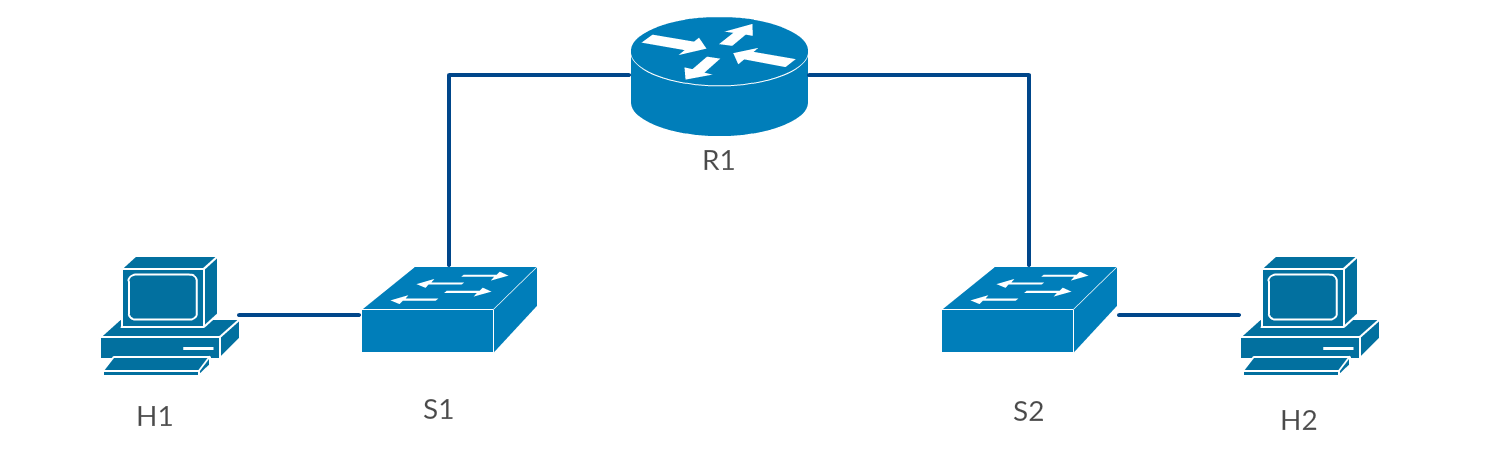
\includegraphics[height=155pt]{img/fig1.png}
    \caption{Mininet Topology}
    \label{fig:topology}
\end{figure}

    \subsubsection*{ Lab Report}
    \begin{itemize}
    	\setlength{\itemindent}{0pt}
    	\item When a packet was sent to a workstation in the other subnet, explain how the source and destination Ethernet addresses were changed.
    	\item What are the source and destination addresses in the IP and Ethernet headers of a packet that went from your machine to the router?
    	\item What are the source and destination addresses in the IP and Ethernet headers of a packet that went from the router to your partner’s machine?
    	\item Answer the above two questions, but now for the echo reply that was returned from your partner’s machine.
    \end{itemize}

\subsubsection*{ Lab Report}
\begin{itemize}
	\setlength{\itemindent}{0pt}
	\item Use the Wireshark outputs from both machines to calculate the average delay that a packet experienced in the router. Note that the system times of the two machines might be different. Show all the steps and submit the Wireshark outputs with your report.
	\item [\(Optional\)] \indent  Compare this value with the previous value in the case of the bridge. Which, a router or a bridge, is faster? Why?
\end{itemize}

\section{Static routing}
  Use what you had learned from previous experiment and config \ref{fig:linearRouters} topology in mininet. Use 255.255.255.0 subnet for all interfaces. \\
  Use ping to test the connections. When you can reach all other subnets successfully, save the routing tables in your workstation and all the routers for the lab report.

\begin{figure}[H]
	\centering
	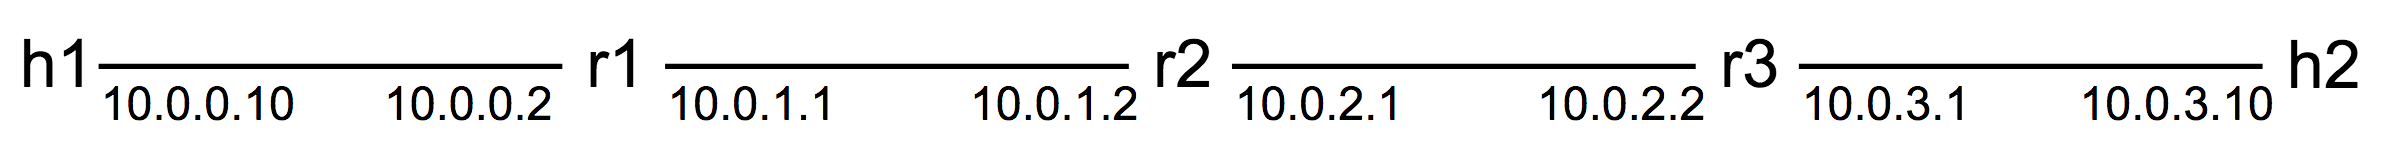
\includegraphics[height=30pt]{img/fig2.png}
	\caption{Mininet Topology}
	\label{fig:linearRouters}
\end{figure}

  \subsubsection*{ Lab Report}
\begin{itemize}
	\setlength{\itemindent}{0pt}
	\item Submit the routing tables of hosts and routers.
\end{itemize}

\section{Traceroute experiment}
In this exercise, we use the same network and configuration of the previous exercises, and use traceroute to find a multi-hop path.
Execute Wireshark on h1 and h2. Then, execute traceroute 10.0.3.10 on h1 to find the route from your host to the h2. Save the output of both traceroute and wireshark.

\subsubsection*{ Lab Report}
\begin{itemize}
	\setlength{\itemindent}{0pt}
	\item Submit what you saved in this exercise.
	\item From the tcpdump output, explain how the multi-hop route was found. Explain the sequence of the ICMP messages used.
\end{itemize}


\section{RIP exercises}
    Create new project in Cisco Packet Tracer and configure topology in Figure \ref{fig:topology} by using 2960 switches and PC (Laptops) in toolbar.

(Use 2960 switch instead of bridge and set of two laptops and one switch instead of each LAN)\\
your configuration must be similar to the Figure \ref{fig:topology} in packet tracer.

\begin{figure}[H]
	\centering
    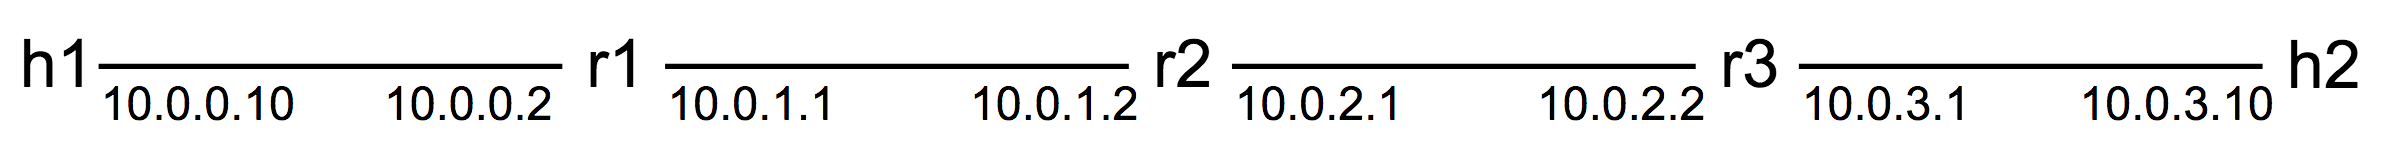
\includegraphics[height=100pt]{img/fig2.png}
    \caption{Implemented Topology in CPT}
\end{figure}

\subsection{Configuring IP address}
	Click  on each laptop and select Config tab then select the FastEthernet0 on the left vertical bar. set IP address for each laptop in 192.168.56.101 to 192.168.56.110 range. \\

	\begin{center}
        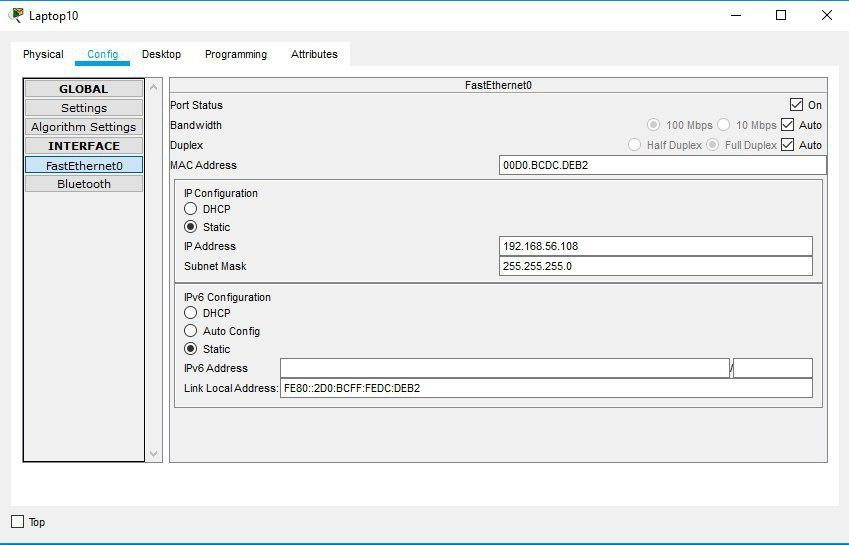
\includegraphics[height=200pt]{img/fig3.png}
    \end{center}
    
    \textbf{Ping} a laptop in LAN D by a laptop in LAN A.

\subsection*{How to Ping}

click on source laptop and select Desktop tab then select command prompt. You can ping destination laptop by its ip. 
\subsection*{Report}
	\begin{enumerate}
		\item show the ping result in your report.
		\item all Cisco command (not required to save graphical image. only report switch or router command)
	\end{enumerate}
    

    %\pagebreak
\subsection{Disabling Spanning-Tree Protocol}
	Click on each switch in your topology and select CLI(Command Line Interface) tab. Enter following commands for disabling STP.
    \begin{itemize}
        \setlength{\itemindent}{50pt}
		\item [Switch>] \textbf{enable}
		\item [Switch\#] \textbf{configure terminal}
		\item [Switch(config)\#] \textbf{no spanning-tree vlan 1-4096}
	\end{itemize}

    \subsection*{Report}
    \begin{enumerate}
        \item Repeat ping process from different source and show the ping result and explain the difference.

    \end{enumerate}
    
    %\pagebreak
\subsection{CLI help}
    Open a random router’s CLI and navigate through User EXEC, Privileged EXEC, Global Configuration and Interface Configuration Modes. In each mode, type ? to display a list of available commands and study these commands.

\subsubsection*{Report}
 Save the output of CLI when you type “?” in each mode and describe one command.
    

    %\pagebreak
\subsection{IP configuration}
    Configure the IP addresses of your workstation and the bridge interfaces as shown in Table 1 and Table 2.\\

    \begin{figure}[H]
        \centering
        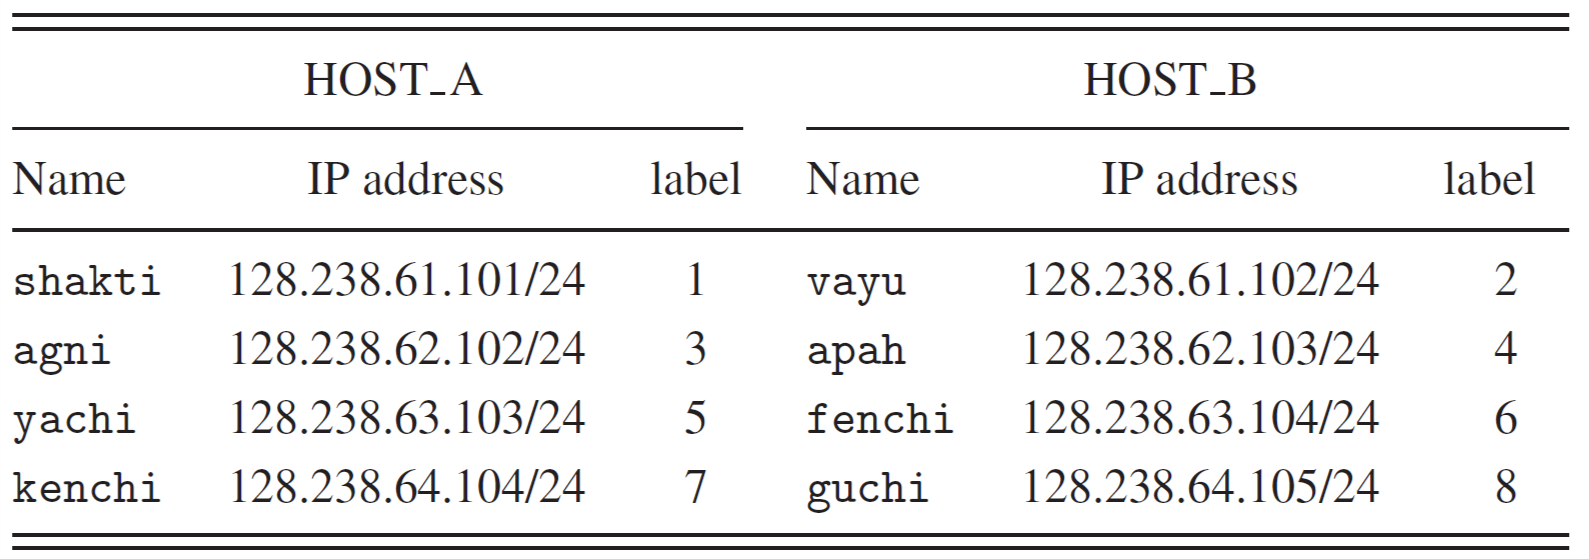
\includegraphics[width=\textwidth]{img/table1.png}
        \caption{Table 1: Host IP addresses}
        \label{tbl:table1}
        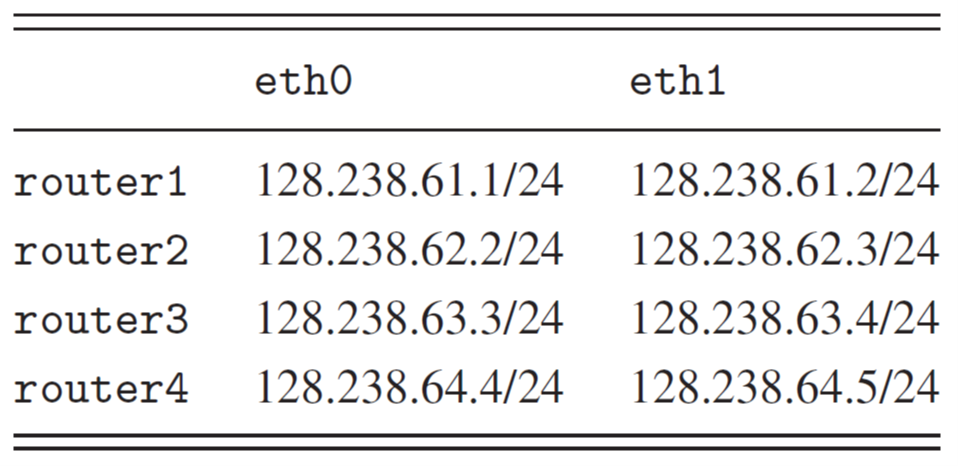
\includegraphics[width=0.6\textwidth]{img/table2.png}
        \caption{Table 2: Router IP addresses}
        \label{tbl:table2}
    \end{figure}

    ping two random hosts and capture ping packet.		

    \subsection*{Report}
    \begin{enumerate}
        \item What are the IP and MAC addresses of a packet that went from Host1 to the bridge? 
        \item What are the IP and MAC addresses of a packet that went from the router to Host2?
        \item Answer the same questions, but for the echo reply that was returned from Host2.
    \end{enumerate}

    %\pagebreak
    
    
        
% \pagebreak
\subsection{Topology Configuration}
   In following Exercise we will use Figure \ref{fig:bridge-ex} as our network topology.You need to change the IP addresses of the bridge interfaces, as well as that of hosts.

\begin{figure}[H]
    \centering
    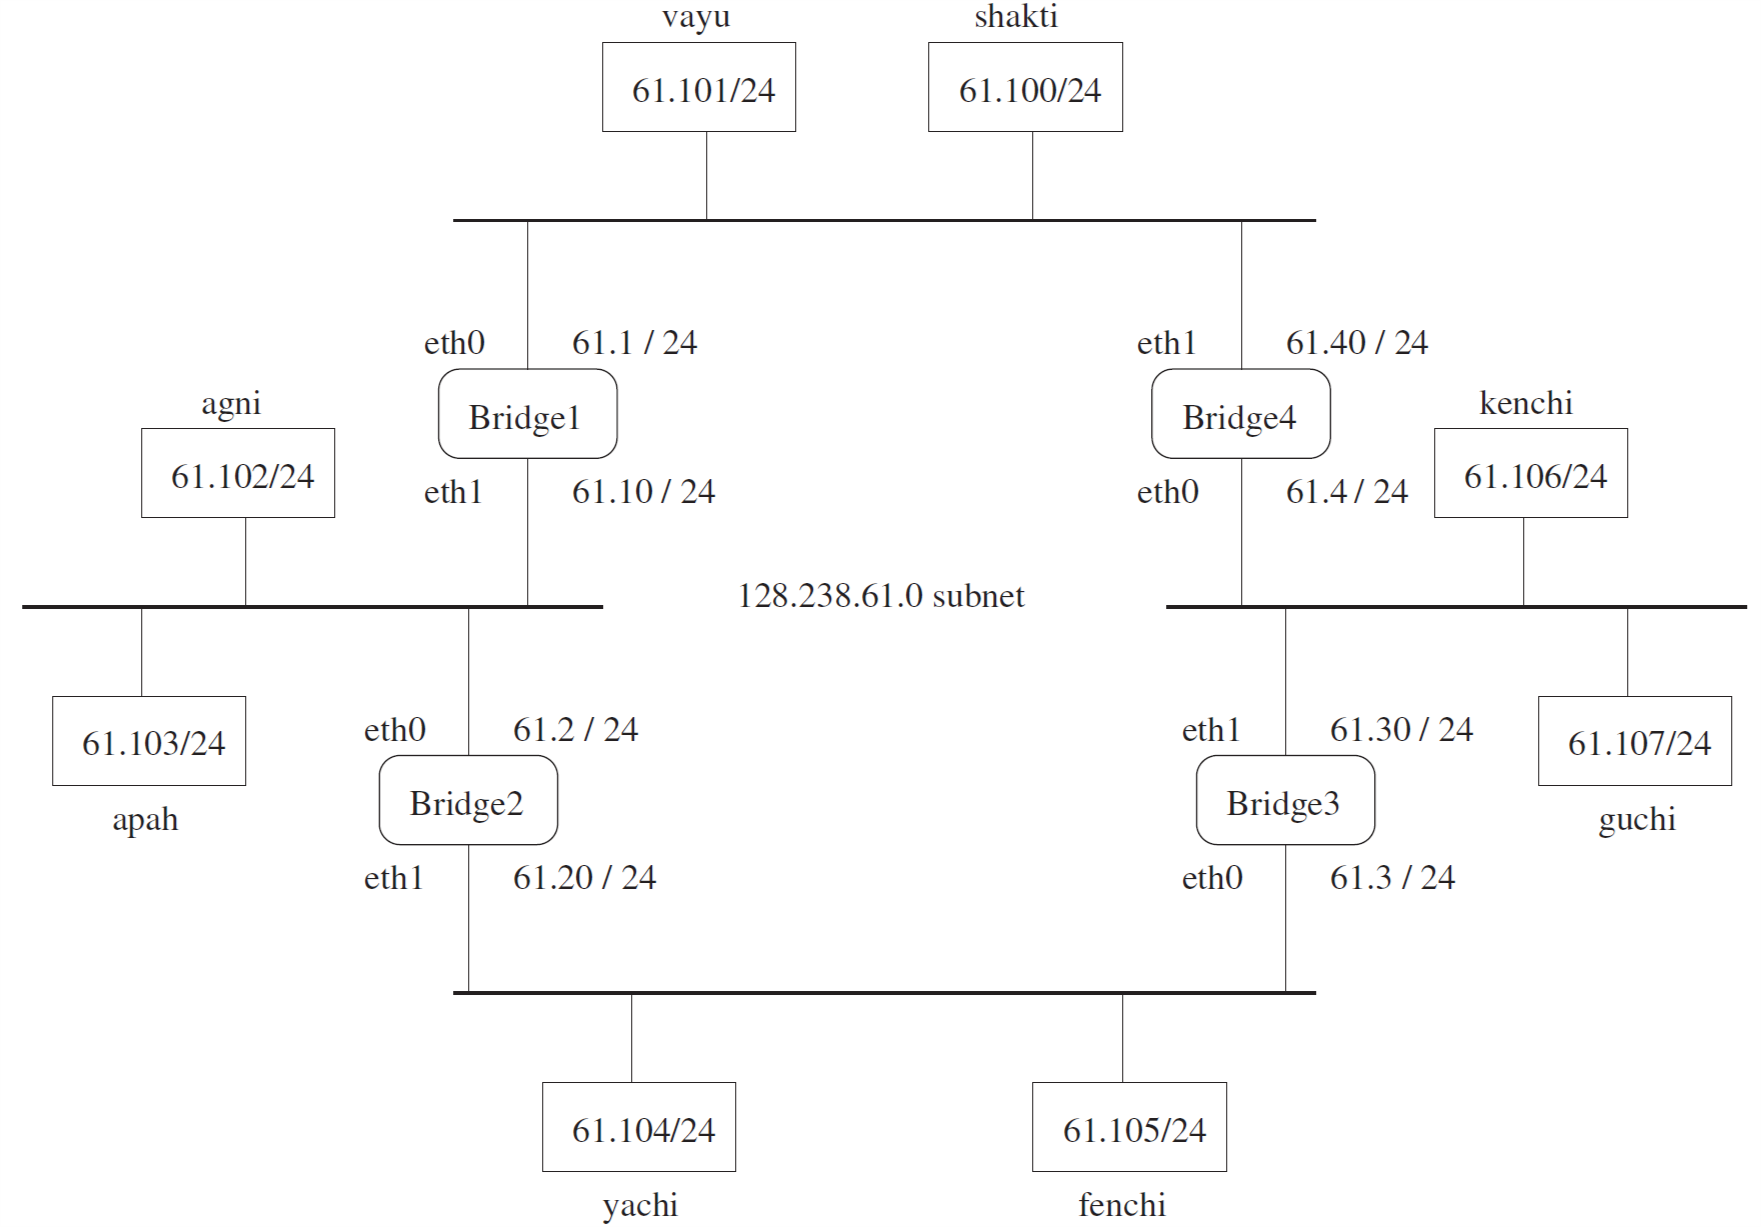
\includegraphics[width=0.8\textwidth]{img/fig4.png}
    \caption{Bridge experiment network}
    \label{fig:bridge-ex}
\end{figure}


\end{document}